%% Cold-start compensation prior. Spliced into taes_fgo_magnav.tex by
%% integrate_coldstart.py. Every number is traceable to a result file in
%% research/gtsam_poc/; the mapping is listed in that directory's README.

\subsection{The compensation prior at cold start}\label{sec:coldprior}
Taken to its per-epoch limit, the smoother exposes a modeling choice that the
full-line batch tolerates. Run from a zero compensation on the cabin
magnetometer with the larger platform field (Mag~4), the incremental smoother at
a \SI{300}{\second} lag leaves the map on four of the five lines, three of the
four counted ones, and ends between \SI{6.6}{} and \SI{27}{\kilo\meter} from
truth, while the same smoother on Mag~5 of the same flights navigates normally
(Table~\ref{tab:incprior}, first column). The asymmetry is the clue, and it is
one of magnitude. Over the first \SI{300}{\second}, the residual against the map
at the INS position is \SIrange{1729}{2081}{\nano\tesla} root-mean-square on
Mag~4 and \SIrange{22}{314}{\nano\tesla} on Mag~5, and the compensation
coefficients that explain the Mag~4 field have magnitudes of
\numrange{552}{722} in the units of Appendix~\ref{app:tl}.

Against that, the priors the model offers for anything other than position are
small. The compensation prior is $\mathbf{P}_0^{\beta}=\mathbf{I}(\sigma_{\beta})^2$
with $\sigma_{\beta}=1$, one scalar shared by all \num{19} coefficients, and the
FOGM disturbance prior is \SI{3}{\nano\tesla}. A cold start on Mag~4 therefore
presents the graph with roughly \SI{2000}{\nano\tesla} that neither nuisance
channel is scaled to explain, and the one remaining degree of freedom that can
absorb it is position, through the map gradient. The single shared
$\sigma_{\beta}$ is the weaker part of that: by Appendix~\ref{app:tl} the
regressor columns range over four orders of magnitude, from direction cosines of
order one to induced and eddy terms carrying the field magnitude, so no single
coefficient scale can be right for all of them.

Table~\ref{tab:priorsweep} measures the sensitivity. Widening $\sigma_{\beta}$
with the prior mean left at zero and nothing else changed removes the divergence
on every Mag~4 line: $\sigma_{\beta}=10$ already suffices and
\numrange{100}{1000} changes the result by up to \SI{14}{\meter}. Replacing the
shared scalar with a per-column prior, one that assigns each basis column a
standard deviation of \SI{100}{\nano\tesla} of measurement contribution rather
than a common coefficient scale, does the same at a physically sized setting: the
Mag~4 lines settle at \SI{19.0}{}, \SI{25.1}{}, \SI{98.9}{}, \SI{30.5}{} and
\SI{23.7}{\meter} and the Mag~5 lines at \SI{12.0}{}, \SI{9.9}{}, \SI{102.7}{},
\SI{16.3}{} and \SI{11.6}{\meter}, with the coefficients left near the magnitudes
the physics implies rather than free to grow by three orders of magnitude as they
do under a uniformly loosened prior. That is the setting we recommend, and it is
the one the rest of this subsection uses. Widening the FOGM prior alone instead,
by a factor of \numrange{10}{100}, recovers three of the five lines and leaves
1003.02 and 1006.08 diverged, which is consistent with the reading above: any
channel wide enough to hold the platform field will do, and the compensation
basis is the channel that should hold it.

We do not claim more than the sensitivity we measured. In particular the
mechanism is not simply that the coefficients cannot reach the platform field:
the window solves of Section~\ref{sec:window1} reach $\|\boldsymbol{\beta}\|_\infty$
of \numrange{544}{795} even at $\sigma_{\beta}=1$, and the prior term at that
magnitude is outweighed by the measurement term by more than two orders of
magnitude. What the tight, dimensionally inconsistent prior does is stiffen the
first linearizations in $\boldsymbol{\beta}$ relative to position, and the
per-epoch smoother commits and marginalizes states while that is true.

Six alternatives can be dismissed by measurement, all at the nominal prior on
line 1007.06 Mag~4 against its \SI{19.5}{\kilo\meter} unless stated. The robust
kernel is not sufficient to explain the failure: removing it entirely gives
\SI{33.0}{\kilo\meter}, and widening the Huber constant from \num{1.345} to
\num{10} and \num{100} gives \SI{18.0}{} and \SI{33.0}{\kilo\meter}, while Mag~5
of the same line returns \SI{11.7}{\meter} with the kernel and \SI{11.7}{\meter}
without it. Map resolution is not sufficient: re-exporting the anomaly grid at
\SI{34}{\meter} spacing instead of \SI{113}{\meter} gives \SI{13.7}{\kilo\meter}.
The lag is not sufficient: at $\sigma_{\beta}=1$, lags of \SI{300}{},
\SI{450}{}, \SI{600}{} and \SI{900}{\second} give \SI{19.5}{}, \SI{14.8}{},
\SI{14.7}{} and \SI{14.5}{\kilo\meter}. Retained linearization is not
sufficient: relinearizing every variable at every update gives
\SI{9.8}{\kilo\meter}. Measurement thinning is not the cause: attaching all ten
raw samples to their nearest kept state gives \SI{22.9}{\kilo\meter}. Nor is the
measurement noise, which is the alternative worth taking most seriously because
the compensated residual on Mag~4 is several times the assumed
$\sqrt{R}=\SI{12}{\nano\tesla}$: setting $\sqrt{R}$ to \SI{65}{} and
\SI{150}{\nano\tesla} across the five Mag~4 lines leaves the divergence in place
and makes it erratic rather than smaller, from \SI{242}{\meter} to
\SI{46}{\kilo\meter} depending on the line, with no line reaching the tens of
metres that widening the compensation prior reaches on all of them. The
$10^{-20}$ conditioning floor on the process noise is likewise not doing the
work: raising it to $10^{-16}$ gives \SI{49}{\kilo\meter} and lowering it to
$10^{-24}$ gives \SI{12.9}{\kilo\meter}. Each of these moves the number and none
recovers the solution, which is what separates a contributing factor from the
one setting that does.

Two measurements bound how far the modeling error reaches. The same graph for
line 1007.06 Mag~4, solved as one full-line batch from the same zero start and
the same nominal prior, reaches \SI{18.6}{\meter}: over a whole line the
compensation has time to move and the map has gradient enough to hold position,
so the cost function itself is sound and the sensitivity is a property of short
spans. The sliding window of Section~\ref{sec:window}, run in this same code
base, sits between the two. At the nominal prior it diverges on 1007.06 Mag~4
(\SI{5430}{\meter}) but not on 1003.02 Mag~4 (\SI{36.6}{\meter}), and seeding its
first window with a ridge fit of the compensation brings 1007.06 to
\SI{30.8}{\meter}, which is the cross-implementation comparison of
Section~\ref{sec:results}-F. The sensitivity is therefore not peculiar to
per-epoch marginalization; it grows as the span each solve sees gets shorter.

A caveat on the divergent runs themselves. The exported anomaly grid covers the
trajectory with a \SI{2.2}{\kilo\meter} margin, and the interpolator clamps
outside it, so once an estimate leaves the grid the map gradient vanishes and no
information can pull it back. The kilometre-scale numbers in the first column of
Table~\ref{tab:incprior} are therefore a floor on how bad the divergence is, not
a measurement of where an unclamped estimator would have gone; what they
establish is that the estimate left the map, not how far.

\begin{figure}[t]
\centering
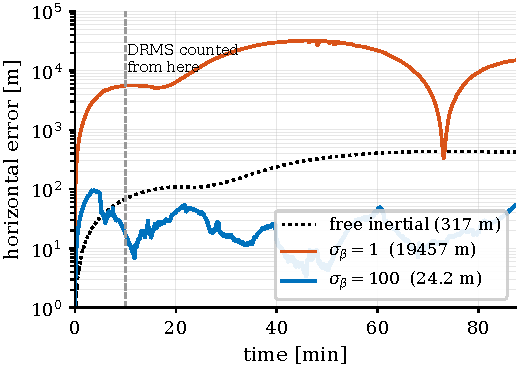
\includegraphics[width=\columnwidth]{figs/fig_prior.pdf}
\caption{Per-epoch smoother on line 1007.06 Mag~4 at a \SI{300}{\second} lag. At
the nominal compensation prior the estimate leaves the map in the first minutes
and never returns; with the prior scaled to the regressor, and nothing else
changed, it stays an order of magnitude below free-inertial drift for the whole
line.}
\label{fig:prior}
\end{figure}

\subsection{The same prior, seen in a single window}\label{sec:window1}
The explanation can be tested one window at a time, which also answers how much
flight the joint problem needs before it is determined. Table~\ref{tab:knee}
reports the solution reached when the same graph is solved as a batch over only
its first $W$ seconds, from a zero compensation, at both priors, with no
commitment and no marginalization anywhere. At $\sigma_{\beta}=1$, the Mag~4
solutions pass through a region, covering at least \SIrange{100}{200}{\second} on
all five lines and extending to \SI{400}{\second} on 1007.06, in which they sit
hundreds of metres to kilometres from truth, while Mag~5 stays within tens of
metres except on the short line 1006.08. At $\sigma_{\beta}=1000$, that region is
gone: every Mag~4 entry outside 1006.08 falls between \SI{2}{} and
\SI{125}{\meter}, and line 1007.02 Mag~4, which at the tight prior never left the
region within the sweep, is at or below \SI{94}{\meter} at every window length.
The single-window and the full-line experiments therefore agree, and they turn on
the same parameter (Fig.~\ref{fig:knee}).

This also fixes what the failure needs. It is not early commitment: these window
solves commit nothing and still land kilometres out. It is a short data span
together with a prior that is not scaled to the regressor. Marginalization only
decides whether the estimator can recover afterwards, and in the fixed-lag case
it cannot.

Line 1006.08 is the exception at both priors. It stays at hundreds of metres
across its middle window lengths and improves only slowly, which is consistent
with the low map-information floor of Remark~\ref{rem:floor} rather than with the
compensation: where $\mathbf{G}\!\approx\!\mathbf{0}$, no prior on
$\boldsymbol{\beta}$ can help.

\begin{figure}[t]
\centering
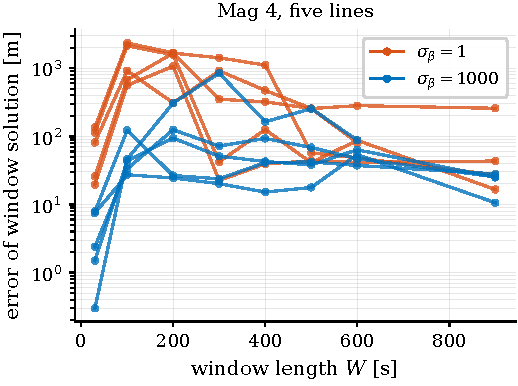
\includegraphics[width=\columnwidth]{figs/fig_knee.pdf}
\caption{Position error of the batch solution over the first $W$ seconds of each
Mag~4 line, from a zero compensation. At the nominal prior the solutions climb to
kilometres over the middle window lengths; at the widened prior the excursion is
absent on every line but the short calibration line 1006.08.}
\label{fig:knee}
\end{figure}

One negative result belongs here because we specifically tested for it. We also
repeated the sweep from a compensation seeded with a ridge fit of
$(z_t-h(\mathbf{p}^{\mathrm{ins}}_t))$ over the same $W$ seconds, to test whether
the far-from-truth solutions are a matter of which minimum the solver selects.
Across the \num{78} combinations of line, magnetometer, and $W$, the two starts
reach objectives that differ at all in only \num{7}; of those, the seeded start
is the cheaper and the more accurate one in \num{5}, and in \num{2} the cheaper
solution is the less accurate one. The window solve is largely indifferent to
where it starts. We therefore do not attribute the cold-start failure to minimum
selection, and we do not claim that the accurate solution can be identified
online by comparing objective values.

\subsection{Real-time cost}\label{sec:realtime2}
With the compensation prior scaled to the regressor, the per-epoch smoother runs
the full breadth at a \SI{300}{\second} lag. Graph states are placed at
\SI{1}{\hertz} rather than at the \SI{10}{\hertz} sample rate, with the
transition compounded and the process noise accumulated exactly over the ten
intervening samples, so the \SI{300}{\second} lag is a \num{300}-state window
updated once a second. Across the ten cases, the update takes
\SIrange{6.1}{10.4}{\milli\second} per state, mean \SI{8.0}{\milli\second}, so an
\SI{87}{\minute} line finishes in \SI{43}{\second} and the margin against the
\SI{1}{\hertz} state cadence is two orders of magnitude. These are mean times on
one core of a laptop-class x86 processor under WSL2, with the measurement factor
evaluated through a Python callback, so they are an upper bound on what native
factors would cost; the corresponding worst cases in the same runs are
\SI{75.5}{\milli\second} per state with full relinearization and
\SIrange{28.7}{35.1}{\milli\second} with all ten raw measurements attached.
Placing states at the full \SI{10}{\hertz} instead makes the same lag a
\num{3000}-state window, which is why a \SI{300}{\second} lag is reported here at
\SI{1}{\hertz} states and not at the sample rate.

The decimation costs the nine measurements dropped between kept states, and on
these lines it does not cost accuracy. The aircraft covers \SI{68}{\meter} per
kept state at the survey ground speed. Attaching all ten raw samples to their
nearest kept state instead of one returns \SI{26.7}{\meter} against
\SI{23.9}{\meter} on line 1007.06 Mag~4 and \SI{26.2}{\meter} against
\SI{19.2}{\meter} on 1003.02 Mag~4, for \numrange{3.5}{3.8} times the
computation. Two things are folded into that comparison and we can separate
neither with the runs we have: the dense variant attaches all ten factors to one
state, so it also assumes a single error state over the \SI{1}{\second} span, and
the measurements themselves are unlikely to be independent at \SI{10}{\hertz}
given that the compensated residual on these lines is several times $\sqrt{R}$. We
report the comparison as a reason not to treat the decimation as a pure loss, not
as evidence about the noise model, which would need an innovation whiteness test
we have not run on these lines.

\begin{table}[t]
\caption{Per-epoch incremental smoother, \SI{300}{\second} lag, \SI{1}{\hertz}
states, at the nominal compensation prior and with the prior scaled per regressor
column (\SI{100}{\nano\tesla} of contribution per column). Smoothed DRMS [m]
after a \SI{600}{\second} warm-up, causal value in parentheses; DRMS is evaluated
at the \SI{1}{\hertz} state grid, and INS is the free-inertial drift computed on
the same grid by the same code. ``div.''\ $>\SI{1}{\kilo\meter}$ and, given the
grid clamping discussed in the text, is a lower bound. Line 1006.08 is the
\SI{14}{\minute} calibration line set aside in Section~\ref{sec:results}; on its
Mag~5 the smoothed estimate is worse than the causal one at both priors, which we
read with Remark~\ref{rem:floor} as the map-information floor rather than as a
smoothing gain.}
\label{tab:incprior}
\centering
\setlength{\tabcolsep}{4pt}
\begin{tabular}{llr rr}
\toprule
Line & Mag & INS & nominal & per column \\
\midrule
1003.02 & 4 & 123.8 & div. & \textbf{19.0} (55.6) \\
1003.02 & 5 & 123.8 & 12.6 (24.4) & 12.0 (21.3) \\
1003.08 & 4 & 271.9 & div. & \textbf{25.1} (47.2) \\
1003.08 & 5 & 271.9 & 10.9 (22.4) & 9.9 (17.3) \\
1006.08 & 4 & 197.7 & div. & \textbf{98.9} (128.4) \\
1006.08 & 5 & 197.7 & 83.9 (52.4) & 102.7 (73.7) \\
1007.02 & 4 & 120.7 & 60.0 (327.8) & \textbf{30.5} (76.9) \\
1007.02 & 5 & 120.7 & 14.0 (40.3) & 16.3 (33.9) \\
1007.06 & 4 & 317.5 & div. & \textbf{23.7} (42.7) \\
1007.06 & 5 & 317.5 & 11.7 (19.8) & 11.6 (16.1) \\
\bottomrule
\end{tabular}
\end{table}

\begin{table}[t]
\caption{Prior sweep on the Mag~4 lines, zero prior mean, no other change:
smoothed DRMS [m] after a \SI{600}{\second} warm-up. The first four columns scale
the single shared coefficient standard deviation $\sigma_{\beta}$; ``per col.''\
instead gives every regressor column a prior of \SI{100}{\nano\tesla} of
measurement contribution; ``$\sigma_S$''\ leaves the compensation prior at
nominal and widens the FOGM disturbance prior a hundredfold instead.}
\label{tab:priorsweep}
\centering
\setlength{\tabcolsep}{4pt}
\begin{tabular}{l rrrr rr}
\toprule
 & \multicolumn{4}{c}{$\sigma_{\beta}$} & per col. & $\sigma_S$ \\
\cmidrule(lr){2-5}
Line & 1 & 10 & 100 & 1000 & 100 nT & $\times100$ \\
\midrule
1003.02 & 26810 & 32.7 & 19.6 & 19.3 & \textbf{19.0} & 33.2 \\
1003.08 & 11262 & 25.7 & 25.0 & 24.5 & \textbf{25.1} & 29.8 \\
1006.08 & 6574 & 117.7 & 99.1 & 85.4 & \textbf{98.9} & 1144 \\
1007.02 & 60.0 & 30.3 & 28.4 & 30.3 & \textbf{30.5} & 56.7 \\
1007.06 & 19457 & 24.1 & 24.2 & 23.9 & \textbf{23.7} & 27.3 \\
\bottomrule
\end{tabular}
\end{table}

\begin{table}[t]
\caption{Solution reached by Levenberg--Marquardt from a zero compensation on a
batch over only the first $W$ seconds of each line: horizontal DRMS [m] over
those $W$ seconds, at the nominal and at a uniformly widened compensation prior.
These are the solutions the solver reaches, not certified global optima. The
free-inertial drift over the same spans runs from \SIrange{0.4}{5.0}{\meter} at
$W=\SI{30}{\second}$ to \SIrange{56.5}{100.7}{\meter} at $W=\SI{900}{\second}$,
so an entry below about \SI{100}{\meter} is at or under the drift it has to beat.}
\label{tab:knee}
\centering
\setlength{\tabcolsep}{3pt}
\begin{tabular}{ll c rrrrrrrr}
\toprule
 & & & \multicolumn{8}{c}{$W$ [s]} \\
\cmidrule(l){4-11}
Line & Mag & $\sigma_{\beta}$ & 30 & 100 & 200 & 300 & 400 & 500 & 600 & 900 \\
\midrule
1003.02 & 4 & 1 & 113 & 2137 & 1569 & 42 & 126 & 41 & 87 & 17 \\
        &   & 1000 & 8 & 27 & 24 & 20 & 15 & 18 & 54 & 11 \\
1003.02 & 5 & 1 & 11 & 42 & 13 & 10 & 9 & 24 & 8 & 11 \\
        &   & 1000 & 12 & 55 & 11 & 12 & 11 & 14 & 16 & 11 \\
1003.08 & 4 & 1 & 20 & 558 & 1069 & 23 & 39 & 44 & 42 & 43 \\
        &   & 1000 & 8 & 123 & 27 & 24 & 41 & 42 & 37 & 28 \\
1003.08 & 5 & 1 & 26 & 70 & 14 & 12 & 24 & 20 & 24 & 22 \\
        &   & 1000 & 3 & 18 & 11 & 3 & 12 & 15 & 11 & 10 \\
1006.08 & 4 & 1 & 81 & 917 & 310 & 915 & 472 & 257 & 81 & -- \\
        &   & 1000 & $<$1 & 46 & 308 & 847 & 164 & 255 & 88 & -- \\
1006.08 & 5 & 1 & 48 & 136 & 341 & 70 & 115 & 50 & 36 & -- \\
        &   & 1000 & 6 & 67 & 113 & 35 & 81 & 26 & 31 & -- \\
1007.02 & 4 & 1 & 136 & 2344 & 1676 & 350 & 321 & 256 & 282 & 258 \\
        &   & 1000 & 2 & 43 & 94 & 51 & 43 & 38 & 63 & 25 \\
1007.02 & 5 & 1 & 13 & 15 & 32 & 34 & 44 & 34 & 60 & 34 \\
        &   & 1000 & 3 & 18 & 22 & 23 & 41 & 37 & 66 & 35 \\
1007.06 & 4 & 1 & 26 & 676 & 1662 & 1420 & 1109 & 57 & 48 & 27 \\
        &   & 1000 & 2 & 33 & 125 & 72 & 93 & 68 & 47 & 25 \\
1007.06 & 5 & 1 & 23 & 78 & 90 & 20 & 17 & 19 & 19 & 12 \\
        &   & 1000 & 1 & 8 & 26 & 11 & 13 & 12 & 10 & 7 \\
\bottomrule
\end{tabular}
\end{table}
